\documentclass{article}
\usepackage{subfig}
\usepackage{graphicx}
\usepackage{color}
\usepackage{hyperref}
\usepackage[ngerman]{babel}
\usepackage[utf8]{inputenc}
\usepackage[T1]{fontenc}




\sloppy
\definecolor{lightgray}{gray}{0.5}
\setlength{\parindent}{0pt}

\begin{document}

\section{Sortierverfahren}

Vergleich der Sortierverfahren selectionSort, mergeSort und quickSort

\subsection{Implementation}
\label{sec:imp}
Die Implementation ist in sort.py zu finden. Die Anzahl der benötigten Vergleiche sind bis zu einer Arraylänge von 50 bzw. 200 Einträgen dargestellt. Wie erwartet ist die Zahl der Vergleiche bei quickSort kleiner als bei selectionSort und etwas größer als bei mergeSort (vgl. Abb. \ref{fig:noc}). Die Wahl der Konstanten ist in Tabelle \ref{tab:func} zu sehen.




\begin{figure}[h!]
\centering
\subfloat[n = 50]{\includegraphics[width=0.47\textwidth]{noc_050.eps}}
~
\subfloat[n = 200]{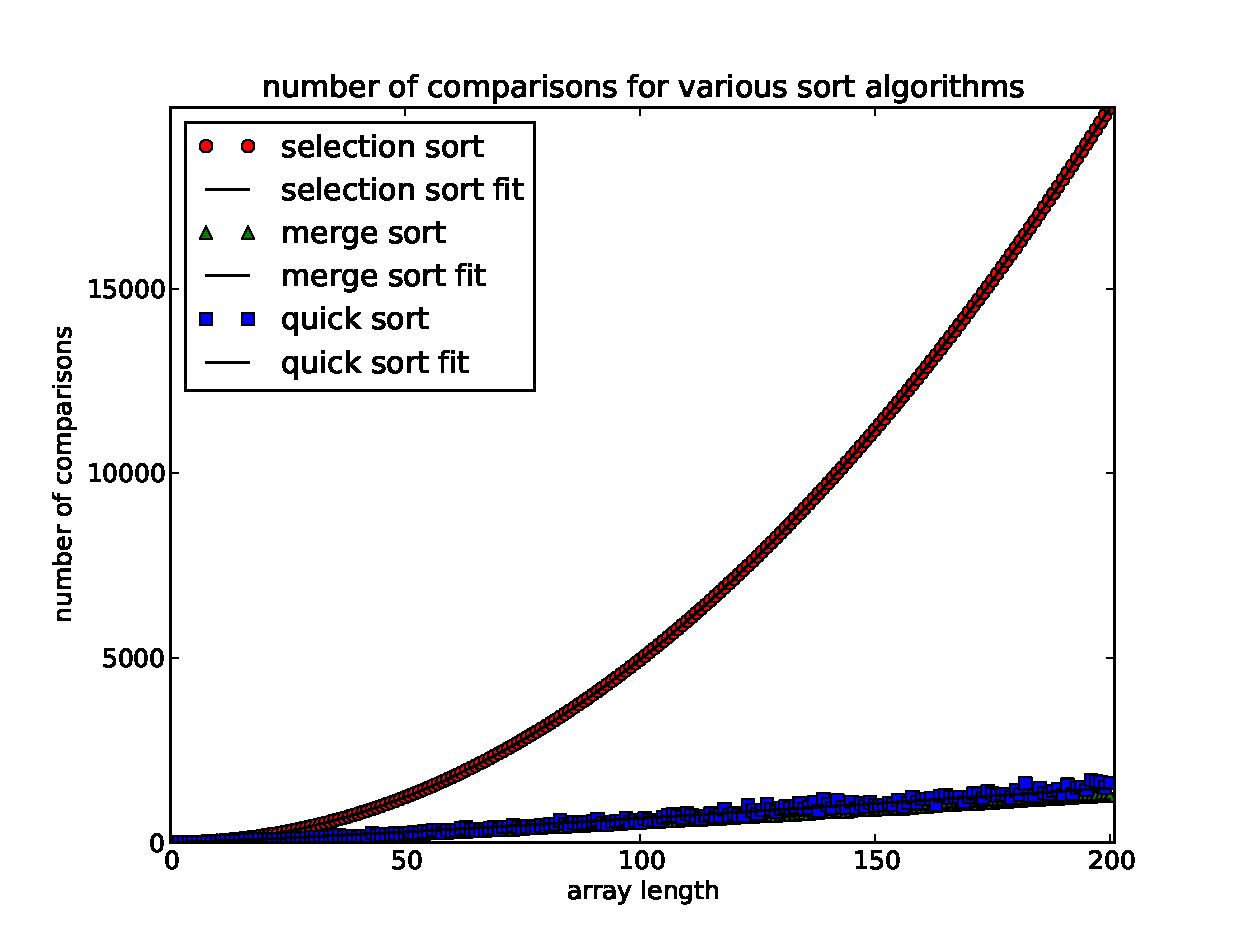
\includegraphics[width=0.47\textwidth]{noc_200.eps}}



\caption{Anzahl der Vergleiche für 50 (a) bzw. 200 (b) Einträge.}
\label{fig:noc}
\end{figure}


\begin{table}[h!]
\centering
\begin{tabular}{|l|l|}
\hline
Algorithmus & Anzahl der Vergleiche \\\hline
selectionSort & $\frac{N^2}{2} -\frac{N}{2}$ \\\hline
mergeSort & $1.1\,N\,\log{N}$ \\\hline
quickSort & $1.2\,N\,\log{N} + N$ \\\hline
\end{tabular}

\caption{Zahl der Vergleiche in Abhängigkeit von der Arraylänge für verschiedene Sortieralgorithmen}
\label{tab:func}
\end{table}

\clearpage
\subsection{Zeitmessung in Abhängigkeit von der Arraygröße}

Die Zeiten für die Sortierverfahren sind bis zu einer Arraygröße von 100 Einträgen in Abb. \ref{fig:time} aufgetragen. Der funktionale Zusammenhang aus \ref{sec:imp} ist hier nicht mehr gültig, da dort nur die Vergleiche gezählt wurden. Tatsächlich muss aber auch noch die Zeit für swaps und das Anlegen neuer Arrays (bei mergeSort) beachtet werden.

Entgegen der Erwartung ist quickSort deutlich langsamer als die anderen Sortierverfahren. MergeSort ist ab ca. 50 Arrayeinträgen schneller als selectionSort.

\begin{figure}[h]
\centering
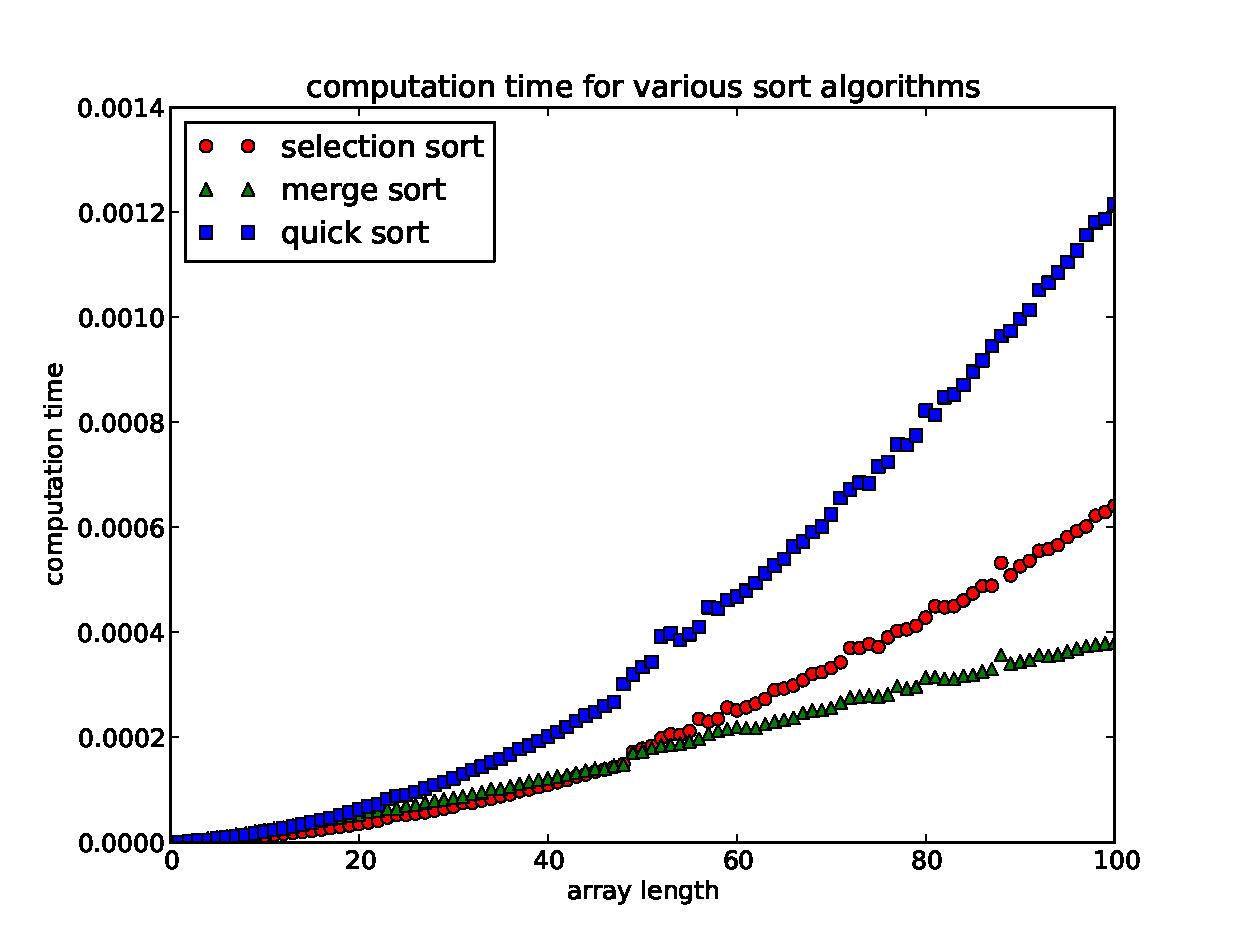
\includegraphics[width=0.8\textwidth]{time_100.eps}

\caption{Benötigte Zeit der Sortieralgorithmen in Abhänigkeit von der Arraygröße}
\label{fig:time}
\end{figure}

\clearpage
\subsection{Überprüfungsalgorithmus}

Der Algorithmus wurde in sort.py als checkSorting implementiert und hat die Richtigkeit der Sortierung bestätigt. Die Überprüfung von Länge, Elementen und Reihenfolge der Elemente ist im Code durch Kommentare gekennzeichnet.

\end{document}
